\documentclass[12pt,letterpaper]{book}
\usepackage[top=2.5cm,bottom=2.5cm,left=3.5cm,right=2.5cm]{geometry}
\linespread{1.3}
\setlength{\parindent}{0pt}
\usepackage{epigraph}
\usepackage{amsmath}
\usepackage{amsthm}
\usepackage{textcomp}
\usepackage{subfigure}
\usepackage{amsfonts}
\usepackage{enumerate}
\usepackage{amssymb}
\usepackage{appendix}
\usepackage[pdftex]{graphicx}
\usepackage{makeidx}
\usepackage{natbib}
\usepackage{algorithmic}
\usepackage{listings}

\setlength\fboxsep{0pt}
\setlength\fboxrule{0.5pt}  
\providecommand{\abs}[1]{\left\lvert#1\right\rvert}
\providecommand{\norm}[1]{\left\lVert#1\right\rVert}
\providecommand{\Real}[1]{\mathfrak{Re}\left(#1\right)}
\providecommand{\Imag}[1]{\mathfrak{Im}\left(#1\right)}

\theoremstyle{definition} \newtheorem{definition}{Definición}[section]
\theoremstyle{plain} \newtheorem{theorem}{Teorema}[section]
\theoremstyle{plain} \newtheorem{lemma}{Lema}[section]
\theoremstyle{plain} \newtheorem{proposition}[theorem]{Proposici\'on}
\theoremstyle{plain} \newtheorem{corollary}[theorem]{Corolario}
\theoremstyle{plain} \newtheorem{remark}[theorem]{Comentario}
\newenvironment{example}[1][Ejemplo]{\begin{trivlist}\item[\hskip 
\labelsep {\bfseries #1}]}{\end{trivlist}}
\newenvironment{dedication}
{
   \cleardoublepage
   \thispagestyle{empty}
   \vspace*{\stretch{2}}
   \hfill\begin{minipage}
        [t]{.3\textwidth}
            \raggedright
}
{\end{minipage}
   \vspace*{\stretch{3}}
   \clearpage
}
\newenvironment{acknowledgments}
{
   \cleardoublepage
   \thispagestyle{empty}
}
{
   \clearpage
}
\makeindex

\setlength{\parindent}{15pt}
\author{Amaury Guti\'errez}
\title{Thesis}

\begin{document}

\frontmatter
\begin{titlepage}

\hfill\\
\hfill\\


\vspace{4cm}

\textbf{ ``Con fundamento en el art\'iculo 21 y 27 de la ley federal del derecho de autor y como titular de los derechos moral y patrimonial de la obra titulada ``WHEN THE EARTH TREMBLES, AUTOMATIC DAMAGE ASSESMENT USING AERIAL IMAGERY'', otorgo de manera gratuita y permanente al Instituto Tecnol\'ogico Aut\'onomo de M\'exico y a la biblioteca Ra\'ul Baill\`eres Jr. Autorizaci\'on para que fijen la obra en cualquier medio, incluido el electr\'onico y la divulguen entre sus usuarios, profesores, estudiantes o terceras personas, sin que pueda percibir por la divulgaci\'on una contraprestaci\'on''}

\vspace{1cm}
\begin{center}
\textbf{Amaury Guti\'errez Acosta}\\
\makebox[2in]{\hrulefill}\\
\textbf{FECHA}\\
\makebox[2in]{\hrulefill}\\
\textbf{FIRMA}\\
\end{center}
\medskip




\end{titlepage}
\endinput 
\begin{dedication}
\large Stay lucky
\end{dedication}
\begin{acknowledgments}
\begin{itemize}
\setlength{\itemsep}{0pt}
\item[-] A Lety por plantar la semilla de lo que soy.
\item[-] A Ricardo por regar esa semilla, no ser\'ia nada sin ti.
\end{itemize}
\begin{center}
\Huge Don't Panic
\end{center}
\end{acknowledgments}

\frontmatter
\tableofcontents
\chapter{Foreword}
It is an inspiring moment for the field of computer vision; machines are now capable of performing tasks that we thought were impossible, reaching new milestones each year. It has been a long time since computers were just large furniture in cold university rooms. Computer power has grown exponentially since those days. In recent years, techniques initially discarded because they were computationally intense are now being unburied and have been showing incredible results in today machines.\\

The objective of this work was to explore the possibilities that these techniques can offer in problems such as damage assessment. In particular, we wanted to teach a neural network how to recognize damaged buildings in aerial imagery. We obtained imagery captured by drones after a massive earthquake stoke south of Mexico in September 2017.\\

This preface serves as an introduction to this work. It gives a short review of the contents of each chapter, and shows how is this dissertation structured.\\

In Chapter 1 we explore our motivations. We expose why our work is essential, and we give a clear explanation about the objective of the experiment. We offer a historical review on the grounds of several natural disasters that have occurred in Mexico, focusing mainly on earthquakes. Additionally, we explore the scope of the project by mentioning limitations and objectives.\\

In Chapter 2 we elaborate an extensive literature review . All the way back to the well-known technique to analyze handwritten digits with the convolutional architecture that started the revolution. A review of modern applications in more complex situations such as object recognition in images. We explore methods to perform damage assessment in the aftermath of natural disasters as it was the primary motivation for this study. We unveil the mathematical details that make this technique to work, diving into the process of backpropagation.\\

In Chapter 3 we discuss on the architecture of our pipeline. This process includes data gathering, data curation, the training of the network and the prediction. We divide the details of the implementation into two parts, client and server side. We delve into the reasoning behind some decisions as the flux of the project suggested new ideas and custom tools emerged. We show our resulting map, and how did we obtain it.\\

In Chapter 4 we examine the development and outcome of our experiment. We evaluate our model against classical computer vision techniques, and we propose a validation scheme for the model using the data at our hands.\\

Chapter 5 dives into the implementation in real-world setting. We use the trained model to predict on orthorectified areas. In the end, the predictions are geolocalised and transformed into human readable adresses, and persisted in a database.\\

Finally, in Chapter 6, we talk about future work, present our observations and discussion points and draw conclusions. We include several improvements that we can address to obtain better results.\\

This work was the result of an internship spent on the Stevens Insitute of Technology (SIT) in Hoboken, New Jersey, during the summer of 2017. I worked under the supervision of Andrea Garc\'ia Tapia, Jos\'e Emmanuel Ramirez Marquez from the SIT, and Raul Sierra Alcocer from the National Commission for the Knowledge and Use of Biodiversity (CONABIO).\\

\mainmatter

\chapter{Introduction}
\epigraph{Good work is not done by `humble' men. (...) A man's first duty, a young man's at any rate, is to be ambitious.}{A Mathematician's Apology \\ G. H. Hardy}
In this chapter, we explore the motivation, objective and scope of the present work.\\


\section{Motivation}

In CONABIO we use landcover maps to analyze and assess the evolution of the environment through time. We make this possible by leveraging classic classification algorithms and a large amount of computing power. While our efforts have been quite productive, these algorithms have certain limits, they rely on the use of the light spectrum. As a consequence, any two categories with similar spectrum footprint will, in all likelihood, confuse the classifier. Curiously enough, humans have little problem distinguish between some of these pairs of categories. For example, crops and grasslands might seem identical to a supervised classifier, but we can certainly tell the difference from one another. This is caused because our brains are not seeing particular pixels and trying to classify them one by one. Instead, our brains look at the whole picture, we focus on zones of the image an all of the information included in them, in other words, we care about context. Convolutional Neural Networks take this into account. Each neuron of the network cares only about a certain zone of the image when information flows through the layers of the network, there are certain neurons that activate upon certain stimuli. Taking context into account lets the network to recognize certain features that would be invisible to a classic classifier, for example: shapes and geometries. When we ask ourselves why it is so easy to differentiate crops from grasslands geometry comes as a natural answer. Crops have very particular shapes.\\

The final objective is to build a comprehensive biodiversity monitoring system. It can be though as two independent efforts. O One of these attemps is the Monitoring Activity Data for the Mexican REDD+ program (MADMex) \cite{rs6053923} which pretends to monitor the behavior of forest and vegetation across the country by processing satelitte imagery. Another effort is the Mexican National Biodiversity and Ecosystem Degradation Monitoring System (SNMB) \cite{GARCIAALANIZ201762} which gathers information about species in the different ecosystems that exist in Mexico.\\

Segnet papers: \cite{DBLP:journals/corr/BadrinarayananK15} in \cite{DBLP:journals/corr/KendallBC15} they enhace their approach by extending their own architecture to include a Bayesian approach. The idea is to add a model of uncertainty to the CNN and use this information to get more acurrate guesses on each of the pixels. They report that this feature adds some improvement in the level of accuracy for many types of architectures not only their own SegNet.


A wonderful introduction to neural networks in the context of remote sensing can be found in \cite{canty2014image}.

In the context of natural disasters other options have been considered \cite{Kryvasheyeue1500779}.\\

DeCAF paper talks about using the features extracted from a neural convolutional network to use in traditional methods. \cite{DBLP:journals/corr/DonahueJVHZTD13}\\

This is another attempt that adds to the evidence that features engineered by the Neural Network work pretty good off the shelf. \cite{DBLP:journals/corr/RazavianASC14}\\

Transfer learning is explored by Yosinski \textit{et al.} \cite{DBLP:journals/corr/YosinskiCBL14}. They propose to use an already trained architecture in new tasks by replacing diferent layers and retraining.\\

In \cite{DBLP:journals/corr/LongSD14} they use the features extracted from the CNN to segment an image.\\

The possibility of having a single model that can perfom correctly in many different tasks is explored in \cite{DBLP:journals/corr/KaiserGSVPJU17}\\

A survey on disctint aspects of how transfer learning is used can be found in \cite{5288526}.\\

The use of active learning together with semisupervised learning tenchniques is explored in \cite{7956153}.\\

Need to take a look into \cite{DBLP:journals/corr/ChenPKMY14}\\

Everardo suggested to look into the U net \cite{DBLP:journals/corr/RonnebergerFB15}.


And the books: \cite{canty2014image}, \cite{richards2013remote}, \cite{tso2009classification} ,\cite{hastie01statisticallearning}

\section{Objective}

It is a wondeful time to explore the use of novel technologies in all types of context. It is in human nature to create tools that revolutionize the way it modifies its envirmonment. We want to explore the use of Convolutional Neural Networks in the context of landcover classification. We believe that this field is very promising and will bloom in the next years. By appliying this methods we hope to obtain results that match the ones that we are already getting with classic methods. In Mexico, the National Institute of Statistics and Geography has been in charge of producing periodical maps about urban settlements in the country. However, it is hard to keep track of irregular settlements and it is often prohibitely costly to create these maps from on-site visits. We want to offer a cheap and innovative alternative to detect and index urban areas using the inexpensive satellite imagery that is available.\\

\section{Scope}

It would be far too ambitious to cover every topic that is involved in the process of the classification using CNNs. We want to explain how do the networks work to a certain extent, but it is not in the scope of this work to untangle every single detail. In the same fashion, the field of Remote Sensing is far too big to be explored in this work. We assume a certain degree of knowledge in related topics and we expose some mathematical details in the appendix. As we already mentioned, the field of Computer Vision is in its climax. Reviewing every single article that has been writen would be a daunting task. We offer a brief literature review that gives some context about the state-of-the art and we hope to build upon ideas and efforts done by a miryad of people. We aimed to built a system capable of procesing imagery and that could be deployed into a cluster for efficient computation. We had in mind to offer a wall-to-wall product of the Mexican landscape.\\


\chapter{Literature review}
\epigraph{If I have seen further it is by standing on the shoulders of giants.}{Letter from Sir Isaac Newton to Robert Hooke}
In this chapter we talk about the state of the art in computer vision and how it has been used for remote sensing problems. We also give a brief account of natural disaster assesment, and how are these machine techniques applied in this sense. We use Sandy Huricane as a study case because of the data that was publicly made available by the NOAA.\\

\section{Computer vision}

 Le Cun \textit{et al.} \cite{lecun} propose to use an architecture of a multi-layer neural network that was able to learn directly from the data with no prior feature extraction. In contrast to the usual path that was used in the context of pattern classification, they created an architecture that was able to automatically extract the features directly from the date without prior manipulation. Instead of using a fully connected network, they proposed a locally connected net. It was capable of extracting local features and passed them down to the subsequent layers in what they called a \textit{feature map}. Each unit took the information of a $5\times 5$ neighborhood of the pixel in the previous layer. The last layer of the architecture consisted of ten units that represented each of the possible digits. This architecture was trained using backpropagation are now known as Convolutional Neural Networks (CNNs). The big leap forward of their result was that their architecture needed very little information about the task it was performing, they where able to extend the use of their method to other symbols, however, they state that the method was not able to be applied to very complex objects. \\


 With the tremendous advances that computer power has suffer in the late years, this has been proven to be incorrect. In 2009 a big image database was gather and published \cite{Deng09imagenet:a}. Ever since this database became the defacto dataset to test classification methods. A few years later, in 2012 Krizhevsky \textit{et al.} \cite{krizhevsky} proposed the use of CNNs in this daunting task.

\section{Remote sensing}


In late years groundbreaking advances in computer vision have had a tremendous impact in other science fields. In particular, we are interested in landcover classification.\\


The use of CNNs in the context of landcover classification was explored by Kussul \textit{et al.} \cite{kussul}. They used an ensamble of CNNs to obtain state of the art results in the classification of different types of crops using multitemporal and multisensor satellite data. They explore 2 aproaches, first they use a 1-D CNN to perform the convolutions in the spectral domain by stacking the different bands from the Sentinel-1 A and La ndsat-8 scenes. This process outputs a pixelwise classification, then they perform a traditional 2-D CNN on the scenes. In order not to lose resolution with the 2-D CNN, they use a sliding window approach assigning the class to the center pixel of the sliding window. Finally, they ensamble both opinions and filter the result to improve the quality of the map.\\

The usual approach with landcover classification is the use of classical classification methods such as support vector machines (SVM) and random forests (RF). In order to improve the performance, features must be handcrafted from the original bands. In \cite{scott}, Grant \textit{et al.} explore the use of Transfer Learning and Data Augmentation in the context of remote sensing images. By exploring well-known high-resolution datasets, they obtain state of the art results.\\

Transfer Learning (TF) is the process of using an already trained CNN, to 

\subsection{Data augmentation}

Data augmentation is a tecnique used to artificially increment the size of the training dataset by appliying affine transformation to the images. It is often used when tagged data is scarce and difficult to obtain. The usual transformations include rotations and relections. When using this tecnique we should be careful about the orientation of the objects, for example a building upside down makes no sense, so there is no use to make the network learn features on objects that it won't see in the wild. Fortunately, aerial imagery don't present this problem. There is no particular orientation that can be considered correct when the pictures are taken from above. This means that we can dramatically boost the size of our dataset.\\

The reasoning behind this idea is that when we see a picture, our brain autmatically orients it into its correct position. By showing the network with different positions and orientations of an object we enrich its knowledge about it.

We can think of the neural network as a newborn kid, in the begining it experiences its environment for the first time



\section{Damage Assessment}




\chapter{System architecture}
\epigraph{We may say, roughly, that a mathematical idea is `significant' if it can be connectted, in a natural and illuminating way, with a large complex of other mathematical ideas.}{A Mathematician's Apology \\ G. H. Hardy}

To analyze a huge amount of images requires a better way of handling and sorting them than just storing them into directories. A set of scripts where built arround a database to let us create trainging and testing sets easilier. Borrowing ideas on how is the transfer learning process made by the engineers in the tensorflow team, our catalog system grew to answer to these needs. In a later stage the analysis process was also included into the system spawning what could become a framework to analyze visual patterns in sets of images with many different purposes.\\

The development process showed the need of a better set of tools to overcome several difficulties that were found. The training stage involved a repetitive process consisting of manually inspecting the available imagery. To this end, a web application was built on top of our catalog system facilitating this process. The process of continuously showing and tagging images proved to be error prone, each mistakenly tagged picture, required to log into the database and delete the wrong entry after maching encoded file names. So a new feature was implemented into our tool, it shows the stored images and their respective tag and lets the user either delete or edit the classification. Finally, when the model was already trained and it was predicting on the orthorectified rasters, the ability to geolocate the predicted damaged areas and place them in a map was very convenient.\\

As it was just exposed, the application was built thinking about the end user. Even though the correct implementation from a design perspective is out of the scope of this work, it was an interesting thing to explore as this would be the kind of problems to be solved in the case of getting such a system into production. The last few paragraphs explained how the system grew to a full server-client architecture to respond to the need of processing data and visualizing the results in a meaningful way.\\

The purpose of this chapter, is to talk about the implementation of our experiment. Details of the pipeline architecture, and the techniques used to obtain and curate data are unveiled.\\

\section{Backend}

To understand why some design decision where made we need to understand the nature of our data. Data came in directories taken from the drones and splitted by flying dates. The quantity and naming of the images was not uniform across towns. Additionaly, drone imagery provide metadata that is useful to geolocate the images. However, this information is limited as it only offers the place where the image was taken but gives no information about the image resolution. This difficulty is overcome with specialized software that takes in the set of images and creates a mosaic using the images using a process known as orthorectification which corrects the distortions caused by the angle in which the image was taken. CENAPRED gave us both resources, the raw drone images and the ortorectified rasters. So the first part of the application was to transform these data into a way that would be easier to manage.\\

Given to previous experience in developing similar projects, it was decided that the system was to be built on top of a Python Web framework. It offers many solutions out of the box, including a familiar line interface set of commands and an object relational mapper that makes the database integration easier. The feature of being ready to offer a web interface was a great plus.\\

\subsection{Data model}

We took advantage of the object relation mapper system that Django offers. In the figure \cite{fig:database} we show a subset of the database diagram. Tables inherent to the features of the Django framework are not shown as they where not modified.\\

The database design was based on reproducible reaseach. We wanted to keep track of the charactistics of the models trained. Also we wanted to know which where the training images used for each model. It was also desirable to be able to reuse models that where trained with different sets of images to benchmark and finally use the best model to actually predict on the orthorectified raster.\\


In order for the tagging application to work, images must be ingested into the system so every time a new sample is tagged we populate the database with information about the original image and the coordinates relative to the original image. In the final stage of the process we produce a list of potential damaged buildings which are also inserted into the database with geografical information and human readable address. We think that this can be helpfull to allocate resources in the most efficient way.\\

\begin{figure}[h]
  \begin{center}
    \subfigure{\label{fig:database}\fbox{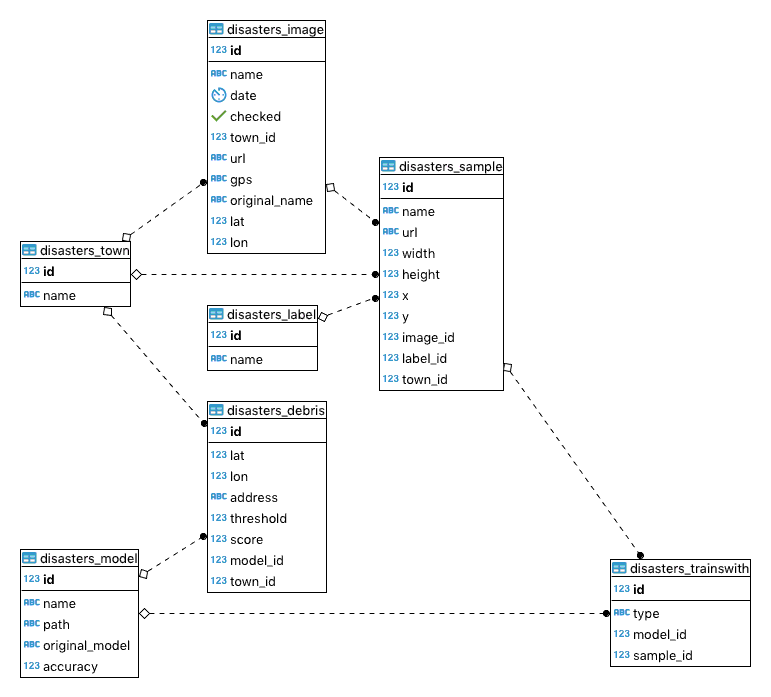
\includegraphics[width=1\textwidth]{images/database.png}}}
  \end{center}
\end{figure}

We built a system to ingest the images from the NOAA service. It lazily downloads the images by checking first if the file is already present in the temporary folder. If the file does not exist it downloads it, then the system tries to add it to the database and persistent file system. To maintain a coherent one to one mapping between the database and the file system, the process of adding a new scene must be successful both in the database and in the filesystem, otherwise, the file is erased from both, and the state of the system remains as it was before the ingestion attempt.\\

\subsection{Tag}


Aerial tagged data is scarce. In particular, for the purpose of our experiment, we don't have any useful metadata on the images. We propose a method to tag samples of the scenes using crowd sourcing. We built a service that crops samples from the images and exposes them to an online application that lets any user with access to tag an image. We have three categories: the image has water in it, the image does not have water in it, and it is not possible to tell. When a positive answer is obtained, the system persists de image in the data base with the information of from which scene was it extracted.\\


\section{Data augmentation}

Given the nature of our task, it is hard to acquire the tagged images. To increment the size of our training dataset, even more, we use a technique known as data augmentation. It relies on the fact that affine transformations do not change the content of the scenes, however, a transformed scene appears as a completely new one to the classifier.\\

The images were rotated by 10 degrees, and reflected by the x-axis and the y-axis this gives us a $x144$ factor, this means that for each tagged image, the training corpus is incremented by $144$ images. The problem with this approach is that when a square image is rotated, some information on the corners is lost so we have to adjust the original image so that we can still crop a complete square from the desired size from it. For our experiment, the input size for the neural network is $227\times 227$ pixels, so the original images must be at least $\sqrt{2}$ times $227$ on each side. This way no matter how we rotate the original image, we can still crop a $227\times 227$ from the center of the rotation without losing any data.\\



\section{Train}

We needed data to train our model. Raw dron images where obtained from the National Center for Disaster Prevention (CENAPRED). Drons flew over three towns in the state of Oaxaca producing $3733$ images during several days. Images contain gps information about the place where they where taken, however, it is not posible to produce a one to one mapping from the pictures to georeferenced points. With this limitation it was not possible to locate possible damaged buildings from the raw images. However, the model does not need any geografical information to be trained as it relies only in the pixel intensities.

Cropping and tagging manualy a large number of samples from the images was prohibitive. In order to overcome this obstacle an online tagging application was developed for this purpose. The idea was to decentralize the tagging procedure by giving an easy to use tool that was able to run from any browser. This way the cumbersome task of tagging the images can be crowdsourced.

By consuming the REST api described in the previous section, a simple web client was developed using jquery and openlayers. The interface is an image viewer with a selection and a button to submit an opition on that the higlighted area. The user will select an appropiate section of the given image, tag it, and then submit the section. In the backend, the image is cropped and ingested into the database.

\begin{figure}[h]
  \begin{center}
    \subfigure{\label{fig:database}\fbox{\includegraphics[width=1\textwidth]{images/visualise.png}}}
  \end{center}
\end{figure}

An additional button is given that lets the user see how well is the current best model performing. The process is quite similar to the previous one. In the server, the image is cropped and then the thumbnail is exposed to the model and the result is written back to the client through the REST api.

\begin{figure}[h]
  \begin{center}
    \subfigure{\label{fig:database}\fbox{\includegraphics[width=1\textwidth]{images/predict.png}}}
  \end{center}
\end{figure}


\begin{figure}[h]
  \begin{center}
    \subfigure{\label{fig:database}\fbox{\includegraphics[width=1\textwidth]{images/submit.png}}}
  \end{center}
\end{figure}

During the process, we noticed that the tagging process can lead to errors. In order to deal with those mistaken tagged images, a visualiser for the tagged images was developed. It consist in a simple interface where the last tagged images are shown with their respective tag. The interface offers a way to delete a given image or just edit the previously assigned tag.

\begin{figure}[h]
  \begin{center}
    \subfigure{\label{fig:database}\fbox{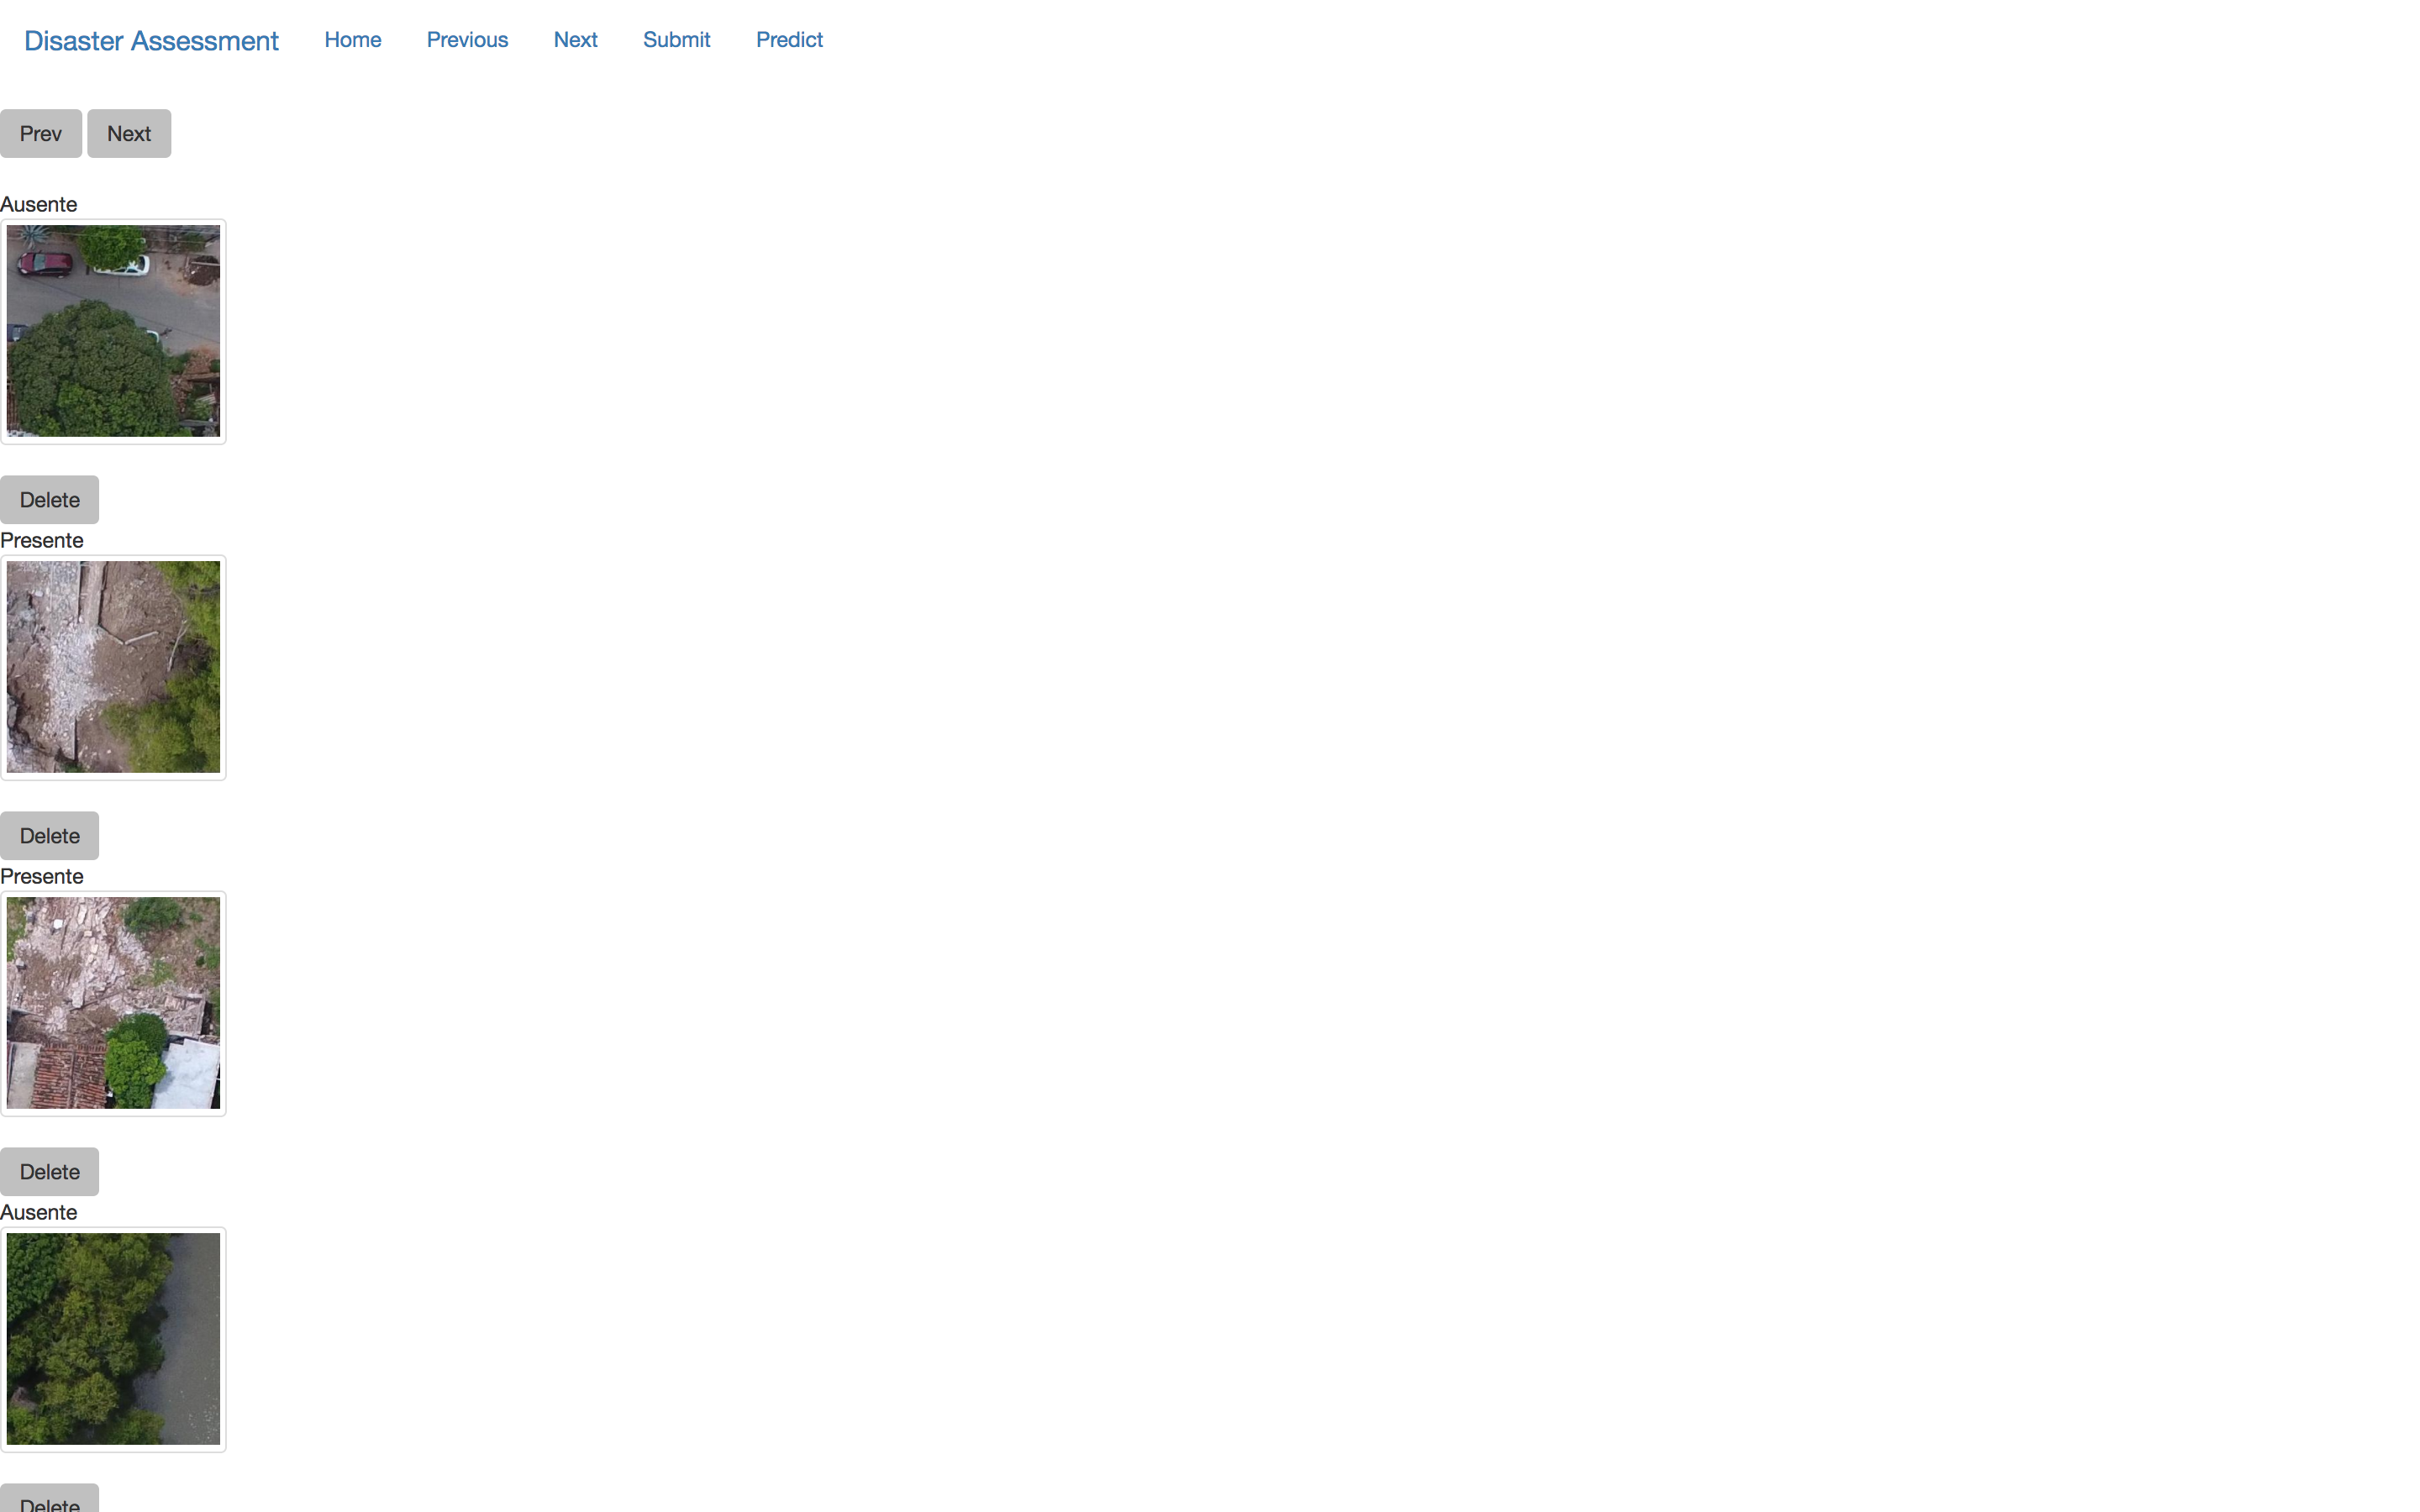
\includegraphics[width=1\textwidth]{images/thumbnails.png}}}
  \end{center}
\end{figure}
Finally, we developed a view for the points that the algorithm finds in the ortorectified image. This view was implemented with open layers and shows information about the location of the potential damaged building in a human readable form. This is done by querying the google api with the latitude and longitude points extracted from the map.

\begin{figure}[h]
  \begin{center}
    \subfigure{\label{fig:database}\fbox{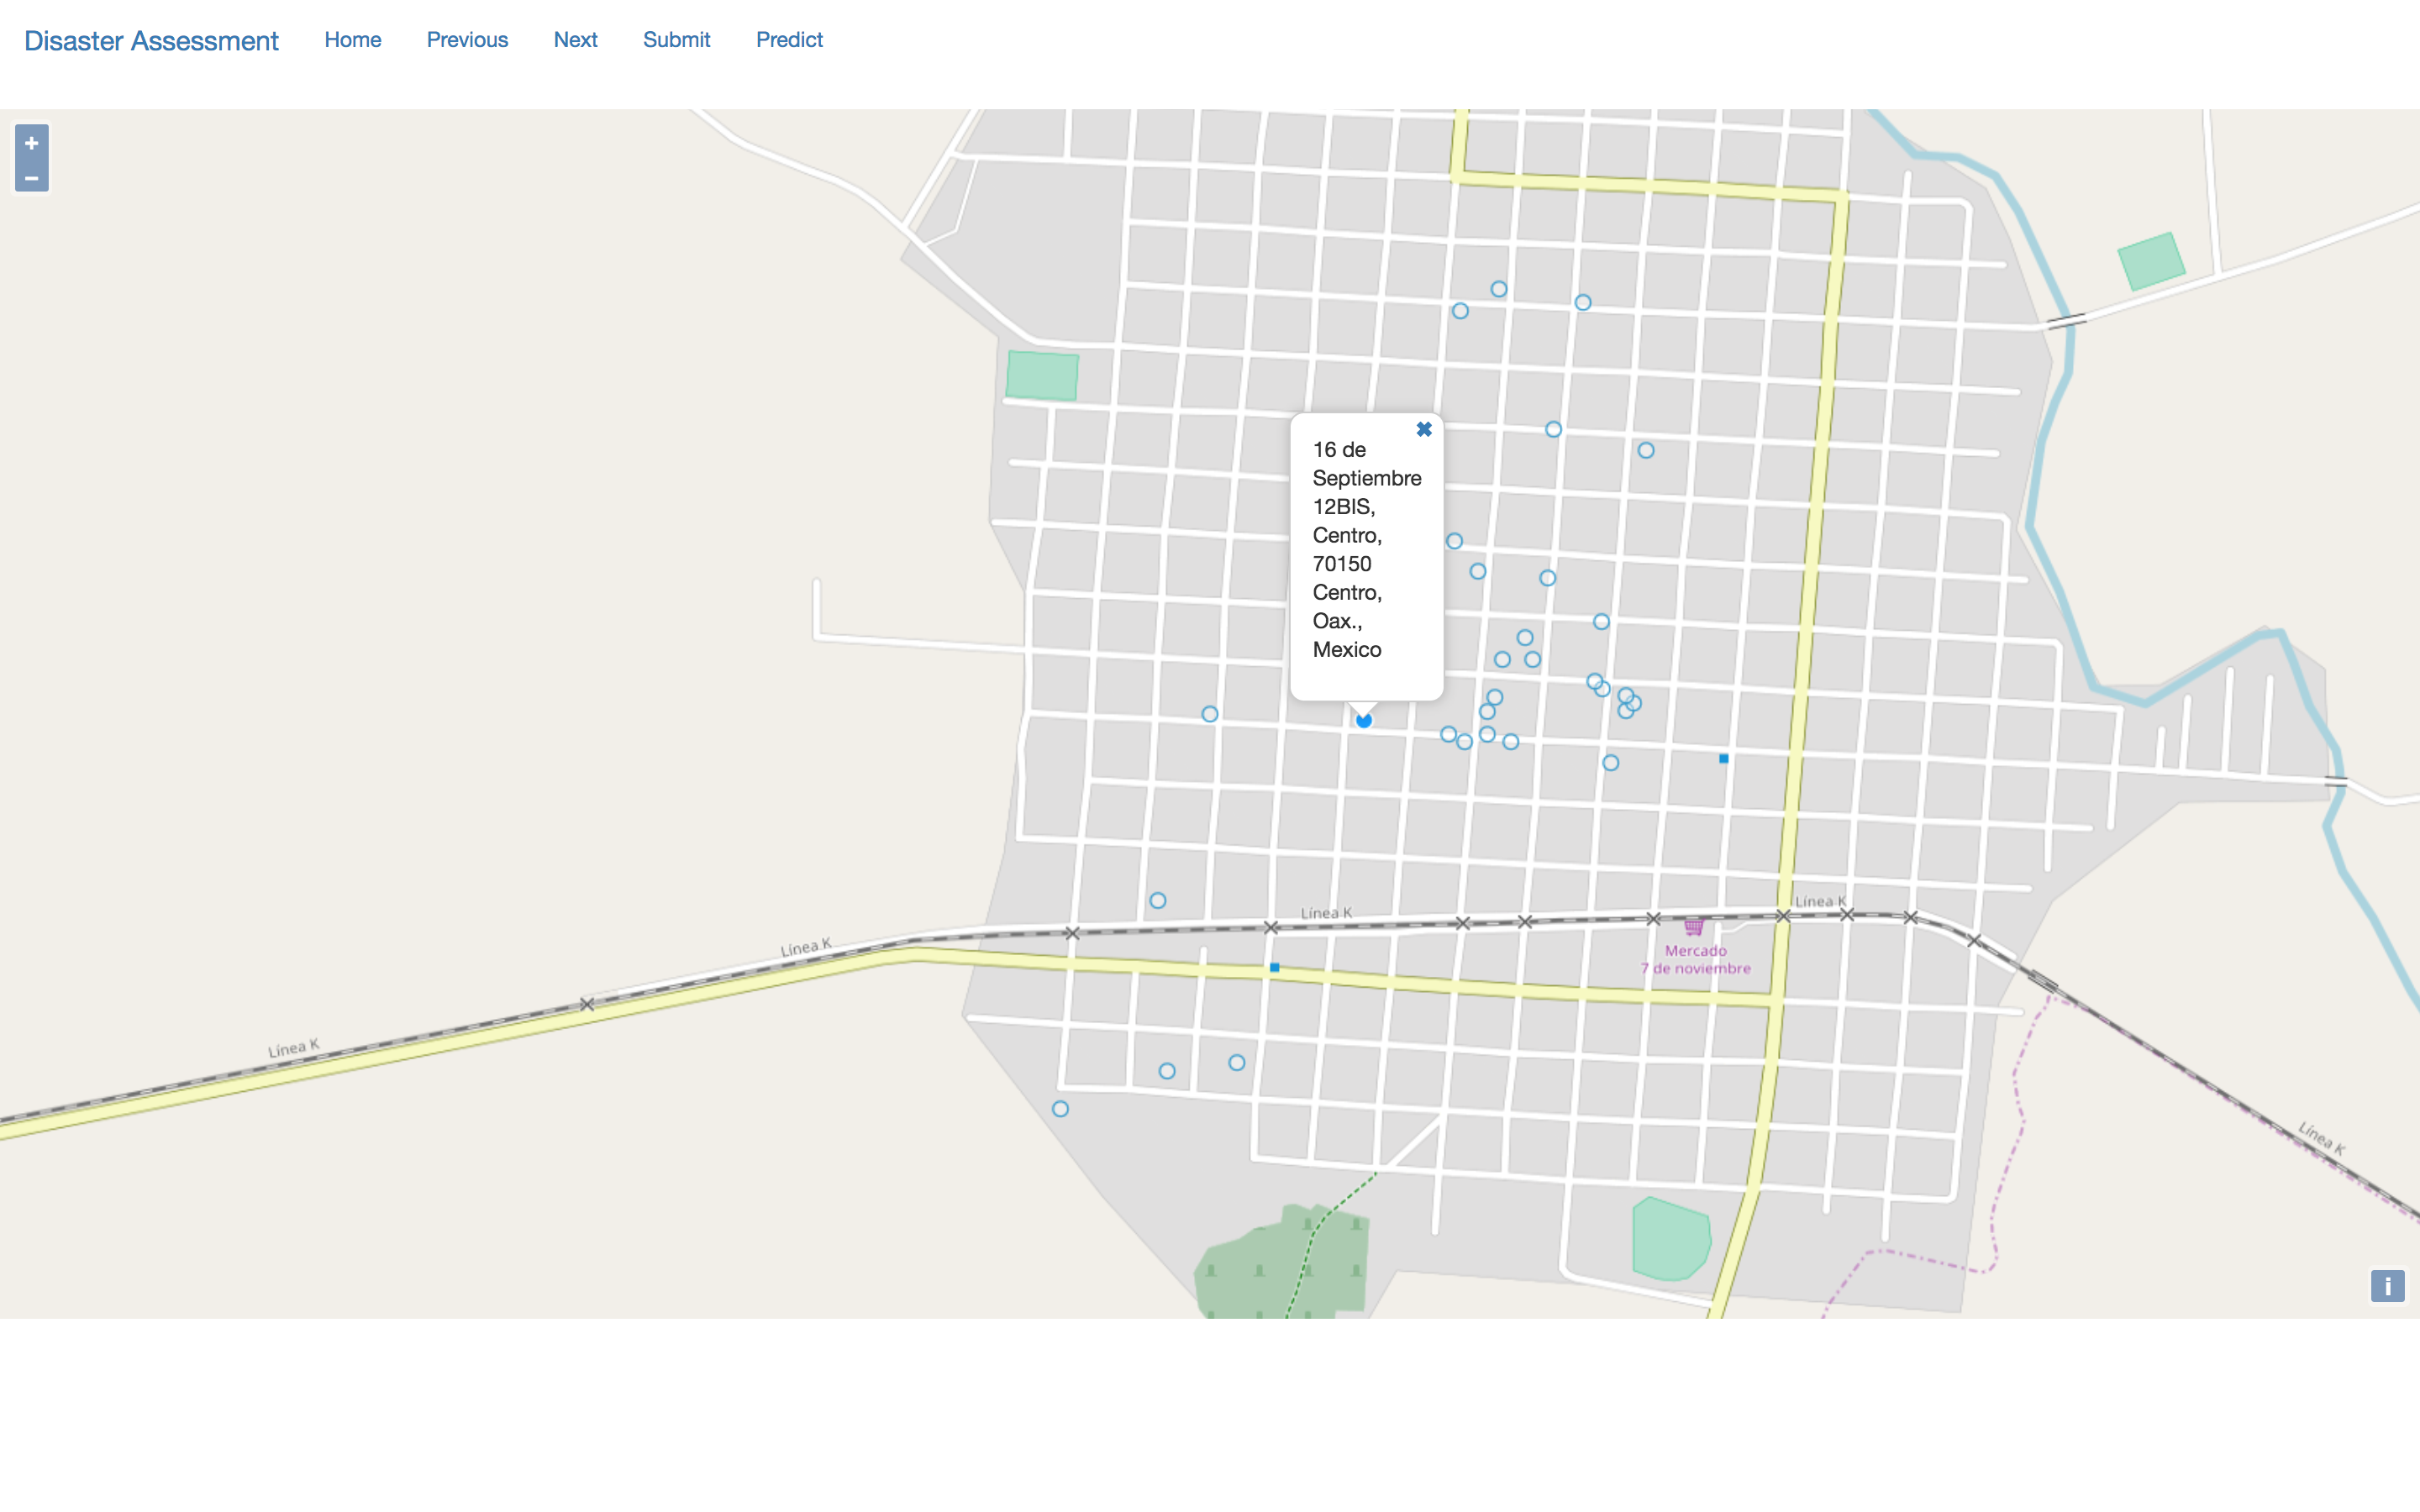
\includegraphics[width=1\textwidth]{images/debris.png}}}
  \end{center}
\end{figure}

\section{Predict}

Another simple front end application was developed to predict on new features, it is very similar to the tagging application. Instead of asking the user about the correct tag, it queries the model and exposes the answer to the front end.\\



\section{Model creation}

In order to create the model we need to select a sample from the thumbnails that we extracted from the original images. We wanted to create a process that was easily reproductible so we would compare models in a simple fashion. To this end the sample must be random each run and we need to split the images in three sets: training, validation and testing.\\

Tensorflow provides a script to retrain the last layer of inception by conecting the extracted features into a sofmax layer, and then training this classifier on the given set. It requires a directory layout tailored built to this purpose. The script was modified to fit our database design in order to make as easy as possible to train several models with homogeneous training, validation, and testing sets.




\chapter{Data analysis}
\epigraph{A mathematical proof should resemble a simple and clear-cut constellation, not a scattered cluster in the Milky Way.}{A Mathematician's Apology \\ G. H. Hardy}
This chapter elaborates on how the model was trained and compared with other techniques from classical computer vision. 

\section{Exploratory analysis}

Drone images from threed different towns in the state of Oaxaca where obtained from the National Center for Disaster Prevention (CENAPRED). This pictures where taken during the week following an earthquake that originated in the Pacific coast of the state. We have 727 images from Santa Maria Xadani, 1872 from Union Hidalgo, and 1134 images from Juchitan of Zaragoza. 


A t-sne analysis was performed with the images, and it is shown in the figure. To this end, the information from the pixels of each images was flattened into a vector comprising the means and standard deviations. This was a simple dimensionality reduction technique and was useful to embed the images into a lower dimensional space. As we can see, images form natural clusters depending on the town that they where taken from. This was somewhat expected because of the light conditions during the exposure tend to have less variance among similar times and places.

\begin{figure}[h]
  \begin{center}
    \subfigure{\label{fig:hausdorff}\fbox{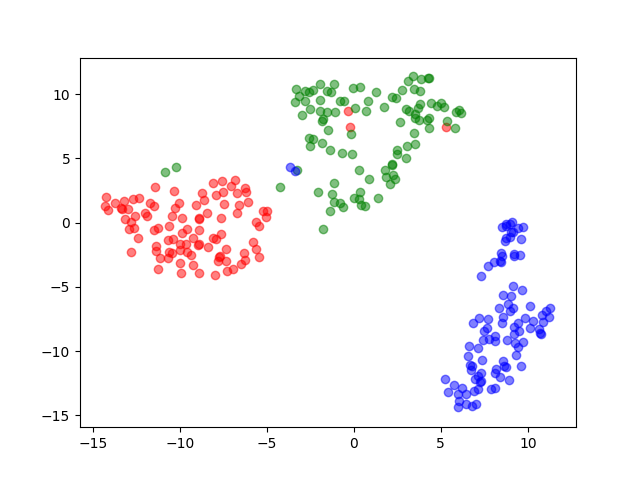
\includegraphics[width=.75\textwidth]{src/t-sne.png}}}
  \end{center}
\end{figure}

The results obtained after applying t-sne, supports the proposed methodology of using images from one town, and try to predict on others. Due to the lack of training data, this was needed to be generated from the sample data. The application detailed in the previous chapter was used to crop and classify $100$ square patches from the images in each of the towns. Each patch was $327\times 327$ and a tag was assigined manualy by the author in each of them.

\section{Model validation}

In order to have an effective algorithm we need that it can perform well in places with images it has never seen before. To test this hipothesis we tried two different methodologies based on cross validation. First of all, classic n-fold cross validation was perform on the pool of training data generated for this experiment. This is, the training set was divided in $n$ subsets and then a model was trained using $n-1$ of those sets while the remaining one was used for testing the model. This was repeated n times leaving a different set each time for testing.

\section{Threshold selection}

The binary classifier assigns a real number in the interval $[0,1]$. To decide which values will be assigined with either level a threshold must be chosen. This was picked using a ROC curve. The ROC curve helps us chosing the performance that fits our needs in the ver possible way. For instance

\section{How much is enough}

In this section we want to create a benchmark on how much images are needed to perform a retraining 

\section{Computer vision versus convolutional neural networks}

\section{Results}


\chapter{A glimpse into the future}
\epigraph{A mathematican, like a painter or a poet, is a maker of patterns. The mathematician's patterns, like painter's or the poet's, must be \emph{beautiful}; the ideas, like the colours or the words, must fit together in a harmonious way.}{A Mathematician's Apology \\ G. H. Hardy}



This was an important experiment because it let us describe the use of novel techniques in the process of image classification.

\section{Conclusion}

Our efforts showed that it is possible to deliver a preliminary product with little training effort. This product might be used as a baseline in the event of a disaster such as an earthquake to give an idea of where to start looking for damaged buildings so resources can be allocated in an efficient manner. 

\section{Drawbacks}

We noticed that, even when the classifier performs well in environments different to the one that it was trained with, it learns to classify dribble, not exactly damaged buildings. We noticed some examples in which the classifier correctly finds scenes with presence of dribble, however, when we inspected the place using Google Street View, we noticed that there was no building in that place. This can can think of two possible scenarios in which this is possible; there was never a building in that place an it was used as a disposal for dribble from other places, or a house was built after the picture in Google Street View was taken. Bothe cases show inherent limitations of the methodology that we are proposing, we can only automate this kind of process to a certain extent.

\section{Future work}

An idea that was beyond the scope of this reasearch was to incorporate a technique known as active learning. In this scheme, the algorithm keeps improving as it receives feedback from the experts. In this fashion, when the model makes mistakes, this incorrectly labeled scenes can be relabeled and feed back to the system in order to create a new model and keep improving its performance. Although there is a limit to the extent in which the algorithm can perform, this might aid in some obvious cases that might not be present in the original training data.

\iffalse

\backmatter
\appendix
\chapter{Appendix A}
chapter a

\chapter{Appendix B}
chapter a

\chapter{Appendix C}
chapter a


\fi

\cleardoublepage
\addcontentsline{toc}{chapter}{Bibliography}
\bibliographystyle{plain}
\bibliography{src/bibliography}
\cleardoublepage
\printindex

\end{document}
